% Changelog (reverse chronological):
% 2026-08-03 08:15 - Claude: v4. Line B's marked lattice point (0,10) turned out
%   to sit exactly on the radius-10 circle (one of the twelve lattice points on
%   x^2+y^2=100: the four axis points and the eight from 6^2+8^2=10^2) -- a
%   coincidence risking the same confusion the v3 fix addressed. Shifted line B's
%   offset from (2,7) to (3,7) (same direction), verified clear of all twelve.
% 2026-08-03 08:05 - Claude: v3, per feedback. The offset lines' own circle
%   crossings don't encode RP^1 direction (a line not through the origin crosses
%   the circle at angles unrelated to its direction). Fixed: added a dashed line
%   through the origin, parallel to each colored line, and moved the square
%   "direction on RP^1" markers to *its* circle crossings (a true antipodal pair).
% 2026-08-03 07:50 - Claude: v2. Thinner lines, distinct colors, marker shapes.
% 2026-08-03 07:35 - Claude: created. First prototype.

\documentclass[tikz,border=3mm]{standalone}
\usetikzlibrary{intersections,calc}

\definecolor{lineAcolor}{RGB}{0,90,181}   % blue
\definecolor{lineBcolor}{RGB}{190,30,30}  % deep red

\begin{document}
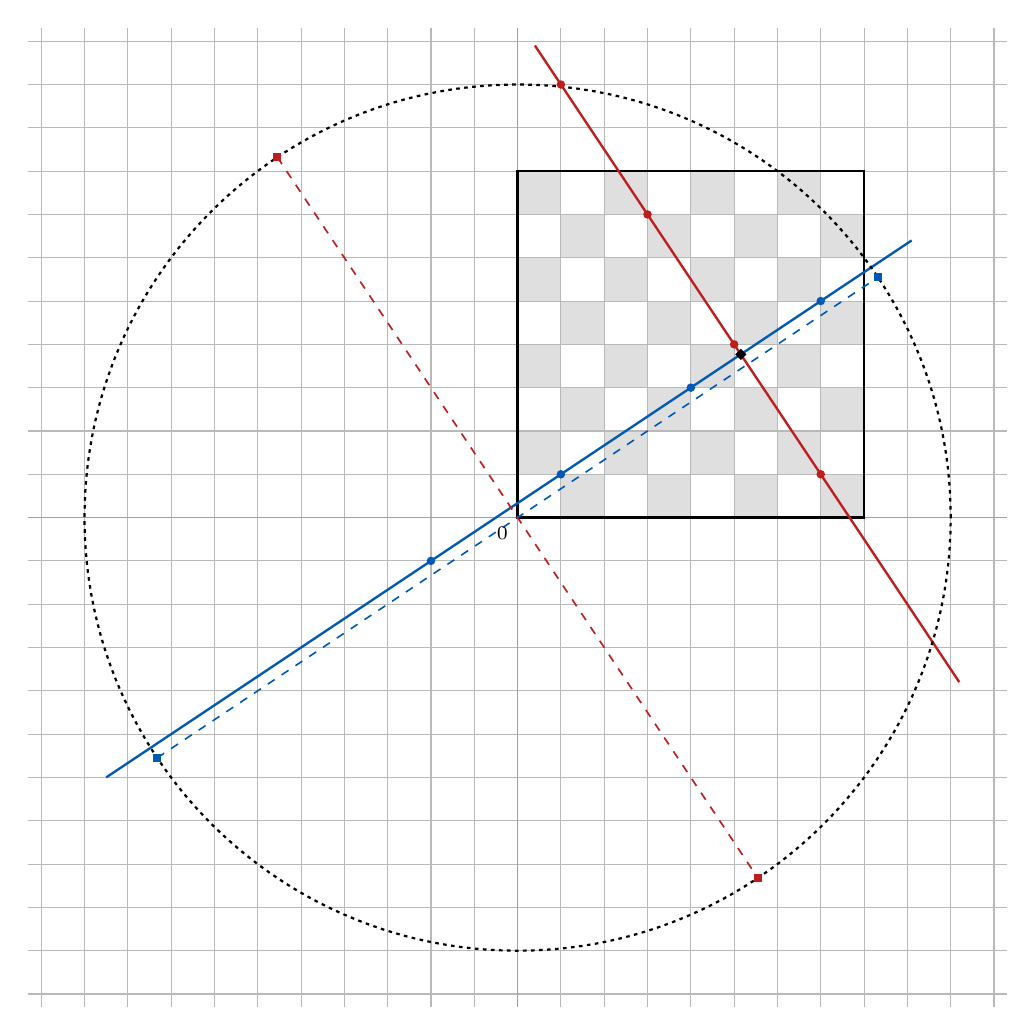
\begin{tikzpicture}[scale=0.55]

  % --- The chessboard: 8x8 alternating squares, corners (0,0)-(8,8) ---
  \foreach \i in {0,...,7} {
    \foreach \j in {0,...,7} {
      \pgfmathparse{mod(\i+\j,2)==0 ? "white" : "gray!25"}
      \edef\sqcolor{\pgfmathresult}
      \fill[\sqcolor] (\i,\j) rectangle ++(1,1);
    }
  }

  % --- Extended integer grid, well past the circle ---
  \foreach \x in {-11,...,11} {
    \draw[gray!55, thin] (\x,-11.3) -- (\x,11.3);
  }
  \foreach \y in {-11,...,11} {
    \draw[gray!55, thin] (-11.3,\y) -- (11.3,\y);
  }

  % --- Axes through the origin, slightly darker than the grid ---
  \draw[gray!75] (-11.3,0) -- (11.3,0);
  \draw[gray!75] (0,-11.3) -- (0,11.3);

  % --- Crisp chessboard border, on top of the grid ---
  \draw[black, thick] (0,0) rectangle (8,8);

  % --- The two actual lattice lines (offset from the origin), thin, colored ---
  % Line A: through (1,1), direction (3,2). t in [-3.5, 2.7] clears the circle.
  \draw[lineAcolor, line width=0.85pt]
    ({1-3*3.5},{1-2*3.5}) -- ({1+3*2.7},{1+2*2.7});
  % Line B: through (3,7), direction (2,-3). s in [-1.3, 3.6] clears the circle.
  % (offset (2,7)->(3,7) vs. earlier versions: (2,7) put the lattice point (0,10)
  % exactly on the radius-10 circle, an avoidable coincidence -- see changelog.)
  \draw[lineBcolor, line width=0.85pt]
    ({3-2*1.3},{7+3*1.3}) -- ({3+2*3.6},{7-3*3.6});

  % --- Auxiliary: the SAME two directions, as lines through the origin ---
  % (dashed, same colors) -- these, not the offset lines above, are what
  % actually cross the circle at the RP^1 direction points.
  \draw[lineAcolor, dashed, line width=0.6pt]
    ({-3*10/sqrt(13)},{-2*10/sqrt(13)}) -- ({3*10/sqrt(13)},{2*10/sqrt(13)});
  \draw[lineBcolor, dashed, line width=0.6pt]
    ({-2*10/sqrt(13)},{3*10/sqrt(13)}) -- ({2*10/sqrt(13)},{-3*10/sqrt(13)});

  % --- Dotted circle, radius 10, centered at the origin ---
  \draw[dash pattern=on 1.3pt off 1.6pt, thick] (0,0) circle (10);

  % --- Direction markers: filled squares where the ORIGIN-parallel lines meet
  % the circle -- a genuine antipodal pair per direction, colored per line ---
  \coordinate (Ap1) at ({3*10/sqrt(13)},{2*10/sqrt(13)});
  \coordinate (Ap2) at ({-3*10/sqrt(13)},{-2*10/sqrt(13)});
  \coordinate (Bp1) at ({2*10/sqrt(13)},{-3*10/sqrt(13)});
  \coordinate (Bp2) at ({-2*10/sqrt(13)},{3*10/sqrt(13)});
  \fill[lineAcolor] ($(Ap1)+(-2.6pt,-2.6pt)$) rectangle ($(Ap1)+(2.6pt,2.6pt)$);
  \fill[lineAcolor] ($(Ap2)+(-2.6pt,-2.6pt)$) rectangle ($(Ap2)+(2.6pt,2.6pt)$);
  \fill[lineBcolor] ($(Bp1)+(-2.6pt,-2.6pt)$) rectangle ($(Bp1)+(2.6pt,2.6pt)$);
  \fill[lineBcolor] ($(Bp2)+(-2.6pt,-2.6pt)$) rectangle ($(Bp2)+(2.6pt,2.6pt)$);

  % --- Lattice points each (offset) line passes through: filled circles ---
  \foreach \p in {(-2,-1),(1,1),(4,3),(7,5)} \fill[lineAcolor] \p circle (2.8pt);
  \foreach \p in {(1,10),(3,7),(5,4),(7,1)} \fill[lineBcolor] \p circle (2.8pt);

  % --- The (non-lattice) crossing point of the two ACTUAL lines: black diamond ---
  \fill[black, rotate around={45:(67/13,49/13)}] (67/13,49/13) ++(-2.6pt,-2.6pt) rectangle ++(5.2pt,5.2pt);

  % --- Origin label ---
  \node[below left, font=\scriptsize] at (0,0) {$0$};

\end{tikzpicture}
\end{document}
